%************************************************
\chapter{Design considerations}\label{ch:design} % $\mathbb{ZNR}$
%************************************************

This chapter provides a general overview of the application's design without explaining implementation details.

Therefore, it will provide a general overview of the application's architecture and point out areas of interest in the design. Concrete implementation details will later be described in \autoref{ch:developer_guide}.

\section{Architectural overview}
\label{sec:architectural_overview}

As the application is a web-application, it was necessary to adjust to the behaviour to the stateless nature of \ac{HTML}. This means every page is mainly self-contained. The only lasting data is provided in the form of a database and a user-session.

Pages communicate parameters via \texttt{POST} or \texttt{GET} requests, when the need arises.

The database is used to store the user logins and product information, whereas the user-session stores the current user and the associated shopping cart.

The overall architecture is focused around providing an abstraction layer between the database and the rest of the code:

\begin{figure}[H]
\begin{center}
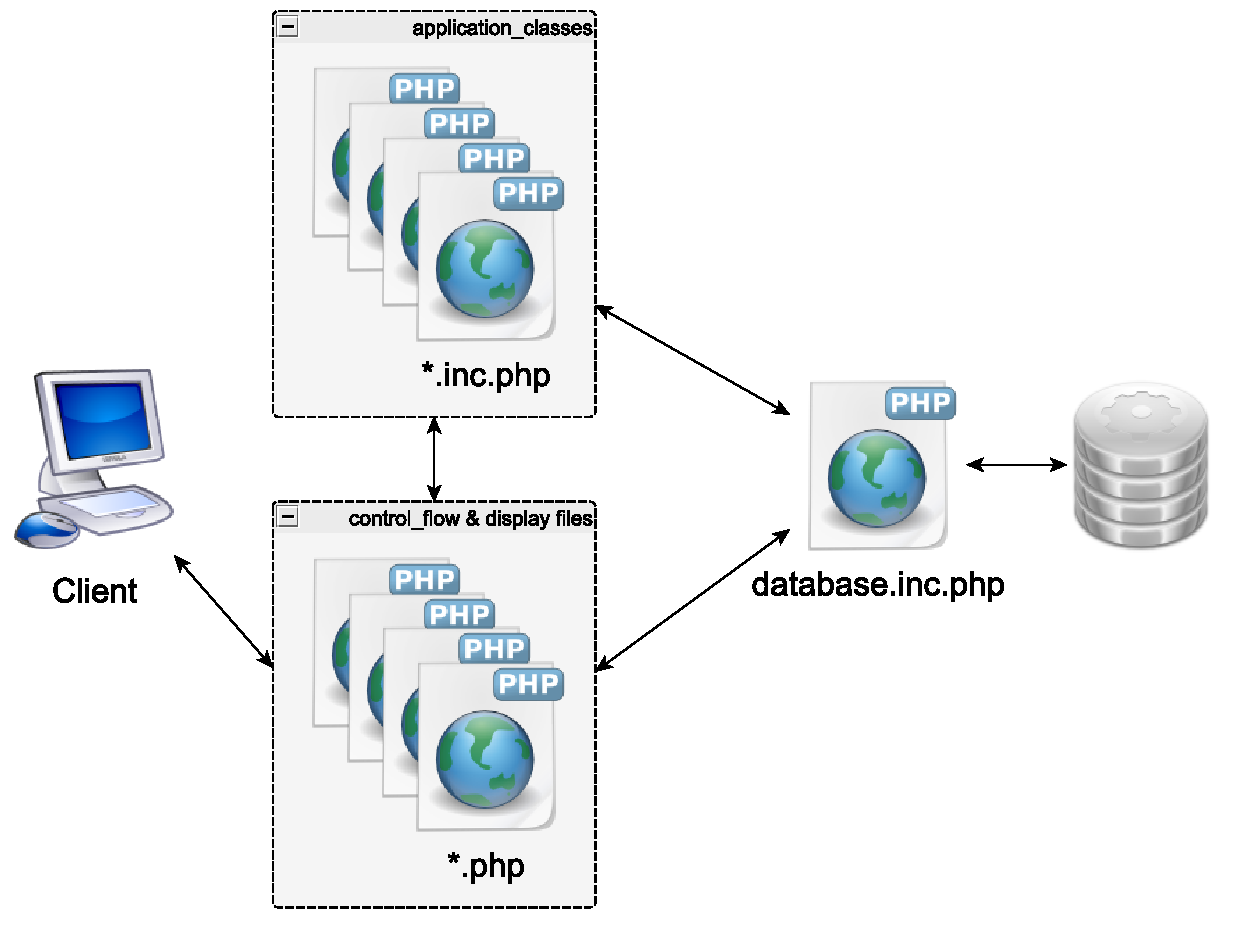
\includegraphics[width=\textwidth]{gfx/overview.pdf}
\caption{Architectural overview}
\label{fig:overview}
\end{center}
\end{figure}

The \texttt{control\_flow} classes are the web pages displayed to the user, whereas the \texttt{application\_classes} are classes that may contain functionality that needs to be reused across different web pages (e.g. the shopping cart)\footnote{Therefore the suffix of \texttt{.inc.php} was used to indicate that these files are meant to be \textit{included} in other php files.}.

This approach was used to ensure the best-practices of \textit{separation of concerns}, as well as \textit{abstraction} and \textit{reuse} of code.
This way - in the best case scenario - only one file needs to be changed when a function needs to be changed. Especially when a different database shall be used only the \texttt{database.inc.php} file would need to be changed.